\documentclass[11pt]{article}

% 02-v5-mcfg-regular-skeletons  (#2骨格MCFG, direction A)
% English source of truth.  Japanese version: japanese/main_JP.tex.
% Provenance of every result: research/README.md.

\usepackage[T1]{fontenc}
\usepackage{lmodern}
\usepackage{microtype}
\usepackage{amsmath,amssymb,amsthm,mathtools}
\numberwithin{equation}{section}
\usepackage{enumitem}
\usepackage{geometry}
\geometry{margin=1in}
\usepackage{booktabs}
\usepackage{tikz}
\usetikzlibrary{arrows.meta,positioning}
\usepackage{cite}
\usepackage{hyperref}
\usepackage{url}
\hypersetup{hidelinks}
\setlength{\emergencystretch}{3em}

\theoremstyle{plain}
\newtheorem{theorem}{Theorem}[section]
\newtheorem{lemma}[theorem]{Lemma}
\newtheorem{proposition}[theorem]{Proposition}
\newtheorem{corollary}[theorem]{Corollary}
\newtheorem{fact}[theorem]{Fact}
\theoremstyle{definition}
\newtheorem{definition}[theorem]{Definition}
\newtheorem{example}[theorem]{Example}
\theoremstyle{remark}
\newtheorem{remark}[theorem]{Remark}
\newtheorem{openproblem}[theorem]{Open Problem}
\theoremstyle{plain}
\newtheorem{mainthm}{Theorem}
\renewcommand{\themainthm}{\Alph{mainthm}}

\newcommand{\Cmcf}[2]{\mathcal{C}^{\mathrm{mcf}}_{#1,#2}}
\newcommand{\D}{\mathcal{D}}
\newcommand{\E}{\mathcal{E}}
\newcommand{\tuple}[1]{\vec{#1}}
\newcommand{\blank}{\square}
\newcommand{\eps}{\varepsilon}
\newcommand{\alphset}{\operatorname{alph}}
\newcommand{\Imp}{\operatorname{Imp}}
\newcommand{\LG}{\mathbf{LG}}
\newcommand{\LI}{\mathbf{LI}}
\newcommand{\SL}{\mathbf{SL}}
\newcommand{\Gp}{\mathbf{G}}
\newcommand{\Dd}{\mathbf{D}}
\newcommand{\ECom}{\mathbf{ECom}}
\newcommand{\LECom}{\mathbf{L}\mathbf{ECom}}
\newcommand{\LT}{\mathbf{LT}}
\newcommand{\LTT}{\mathbf{LTT}}
\newcommand{\ACom}{\mathbf{ACom}}
\newcommand{\Com}{\mathbf{Com}}
\newcommand{\ttyp}{t_{\mathrm{typ}}}
\newcommand{\bth}{\bar\theta}
\newcommand{\Kocc}{K_L}

\title{Which Regular Skeletons Give Polynomial Characteristic Data\\
for Multiple Context-Free Languages?}
\author{Takayuki Kuriyama}
\date{Draft, 23 November 2026}

\begin{document}
\maketitle

\begin{abstract}
In distributional learning of multiple context-free languages from positive
data under a fixed finite-semigroup typing $s$, the total length of
characteristic data is controlled by the \emph{representative length}
$\tau(G,s)$ of a target presentation $G$: the length of a shortest tuple that
has the same type and the same distribution as a given typed nonterminal.
For typings whose image is a local group (pseudovariety $\LG$), $\tau$ is
polynomial in the size and thickness of $G$ at every fan-out, and at fan-out
one $\LG$ is exactly the boundary for typings.  Outside $\LG$ almost nothing
was known beyond fan-out one.

We study the question from the side of the target.  A target is described by
a regular \emph{skeleton} $R$ together with arbitrary additive counting
conditions on factors of bounded length.  We prove that if every local monoid
of the syntactic semigroup of $R$ has commuting idempotents, i.e.\ the
syntactic semigroup lies in $\LECom$, then for every fixed fan-out and rank
the representative length is polynomial in the number of nonterminals and the
thickness of any reduced good presentation, for every typing that refines the
content, a fixed window and the syntactic morphism of $R$, provided the target
is substitutable for that typing.  These typings are in general outside $\LG$.
The proof decorates every letter with the state of a fixed automaton whose
transition semigroup is a local group, transfers the target to a locally
counting language over the decorated alphabet, and applies a pigeonhole and
Euler-rerouting argument for locally counting languages.  The skeletons for
which such a decoration recovers the full syntactic value from every entry
are exactly those with syntactic semigroup in $\SL*\LG$, and we show
$\SL*\LG=\LECom$.  We also show that the method stops exactly there: for
skeletons outside $\LECom$, no local-group decoration followed by any local
counting condition determines membership, and three minimal examples are
given.  The boundary on the side of typings ($\LG$: local monoids are groups)
and the boundary on the side of skeletons ($\LECom$: local monoids have
commuting idempotents) are thus both conditions on local monoids.
\end{abstract}

\tableofcontents

%======================================================================
\section{Introduction}
\label{sec:intro}

\paragraph{Background.}
Distributional learning infers a grammar from the contexts in which strings
occur.  Clark and Eyraud \cite{ClarkEyraud2007} showed that substitutable
context-free languages are identifiable in the limit from positive data with
polynomial resources, and Yoshinaka \cite{Yoshinaka2011} extended this to
multiple context-free languages (MCFLs) \cite{SekiEtAl1991} with
multidimensional substitutability; see \cite{ClarkYoshinaka2014,ClarkYoshinaka2016}
for surveys and extensions, and \cite{Yoshinaka2015General} for a general
algebraic perspective.  Efficiency of such learners is measured by the update
time and by the size of characteristic samples
\cite{deLaHiguera1997,EyraudHeinzYoshinaka2016}.

In the companion work \cite{KuriyamaTCS1,KuriyamaMCFGpreprint,KuriyamaCompendium}
the learner is biased by a fixed finite-semigroup typing
$s:\Sigma^+\to\mathsf S$: two tuples are compared only if their components have
equal $s$-types.  The class $\Cmcf{f}{s}$ of $(f,s)$-tuple-substitutable
$f$-MCFLs contains every regular language recognized by $s$, and grows with
$s$.  The cost of this generality is measured by the total length of
characteristic data.  A reduced good presentation $G$ of the target has a
\emph{representative length} $\tau(G,s)$: for each realized typed nonterminal
$X$, the length of a shortest tuple equivalent to the yields of $X$ (same type,
same distribution), maximized over $X$.  Characteristic data of total length
$O(N_{\mathrm{typ}}(1+\bth_G+r\tau(G,s)))$ exist (Fact~\ref{fact:char-data}),
so a polynomial bound on $\tau$ in the size and thickness of $G$ gives
polynomial characteristic data.

On the side of \emph{typings} the picture is as follows.  If $s(\Sigma^+)$ is a
local group (every local monoid $e\mathsf Se$ is a group, pseudovariety
$\LG$), then the typed yields themselves are short at every fan-out
\cite{KuriyamaCompendium}.  At fan-out one, $\LG$ is exactly the pseudovariety
boundary: every typing onto a semigroup outside $\LG$ admits targets whose
characteristic data are exponential \cite{KuriyamaTCS1,KuriyamaTypingClass}.
At fan-out at least two, whether $\LG$ is still the boundary is open
(Open Problem~\ref{op:fanout-two}).

\paragraph{This paper: the side of the target.}
Instead of restricting the typing, we restrict the target.  A target is
described by a regular \emph{skeleton} $R$, through its syntactic morphism
$\rho_R$, together with arbitrary additive conditions on the counts $N_\ell(w)$
of factors of a fixed length $\ell$.  The typing is required to see the
content, a fixed window and $\rho_R$; it is in general not in $\LG$.

\begin{mainthm}[Main theorem; Theorem~\ref{thm:main}]
\label{thm:A}
Let $R\subseteq\Sigma^+$ be regular with syntactic semigroup in $\LECom$, i.e.\
in every local monoid of $\Sigma^+/{\sim_R}$ any two idempotents commute.  Fix
$\ell,f,r\ge1$.  Suppose that membership of positive words in $L$ depends only
on $(\rho_R(w),N_\ell(w))$, that $s\preceq(c_\Sigma,b_\ell,\rho_R)$, and that
$L\in\Cmcf{f}{s}$.  Then every reduced good fan-out-$\le f$, rank-$\le r$
presentation $G$ of $L\cap\Sigma^+$ satisfies
\[
  \tau(G,s)\le\mathrm{poly}(v,\bth_G),
\]
where $v$ is the number of nonterminals and the degree depends only on
$R,\Sigma,\ell,f$.  Consequently $L$ has characteristic data of polynomial
total length.
\end{mainthm}

Here $c_\Sigma$ is the content typing and $b_\ell$ the window typing that
records the first and last $\ell-1$ letters.  The typings in
Theorem~\ref{thm:A} are outside $\LG$ as soon as $|\Sigma|\ge2$
(Lemma~\ref{lem:window-not-lg}).  The hypothesis on $R$ is satisfied, for
instance, by all locally threshold testable languages, all group languages,
and the language of words in which every maximal $\mathtt a$-run has even
length, whose syntactic semigroup is the symmetric inverse monoid $I_2\notin\LG$
(Example~\ref{ex:running}, our running example).

\paragraph{Method.}
The proof has three layers (Figure~\ref{fig:layers}).
\begin{enumerate}[label=(\arabic*),leftmargin=*]
\item \emph{Locally counting targets} (Theorem~\ref{thm:L}).  If membership
depends only on the window type and the factor counts, a pigeonhole argument on
frequencies of de Bruijn edges, colours of impure windows along a depth-first
traversal, and Euler rerouting with frozen blocks yield short equivalent
representatives.
\item \emph{Decoration} (Theorem~\ref{thm:B}).  Decorating every letter with the
state of a fixed automaton turns a skeleton into a locally counting language
over a larger alphabet.  The decorated presentation is again reduced and good,
and its thickness stays polynomial provided the transition semigroup of the
automaton is a local group; the original distribution is recovered by
projection.
\item \emph{Algebra of skeletons} (Theorem~\ref{thm:C}).  A skeleton admits a
local-group decoration from which its full syntactic value can be read off
from every entry if and only if its syntactic semigroup lies in $\SL*\LG$, and
$\SL*\LG=\LECom$.
\end{enumerate}

\begin{figure}[t]
\centering
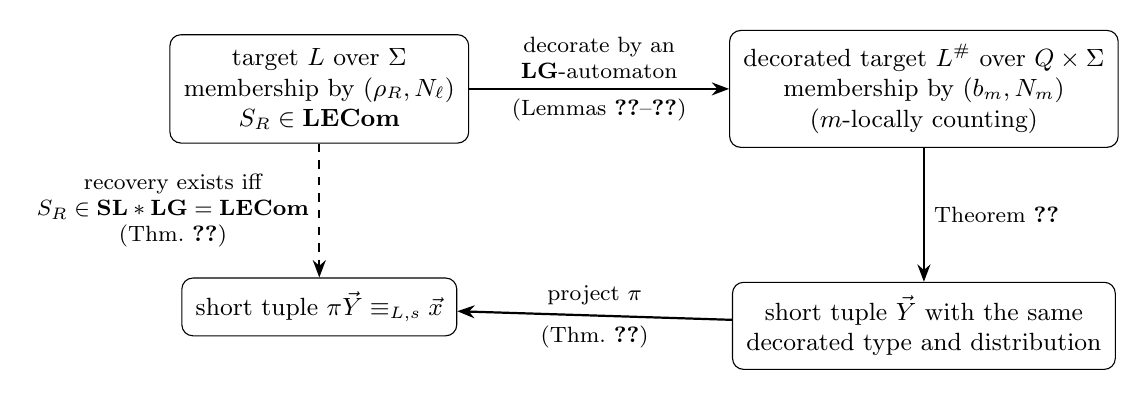
\begin{tikzpicture}[
  box/.style={draw,rounded corners,align=center,inner sep=5pt,font=\small},
  arr/.style={-{Stealth[length=2.2mm]},thick},
  lab/.style={font=\footnotesize,align=center}]
\node[box] (L) {target $L$ over $\Sigma$\\ membership by $(\rho_R,N_\ell)$\\ $S_R\in\LECom$};
\node[box,right=3.3cm of L] (Ld) {decorated target $L^\#$ over $Q\times\Sigma$\\ membership by $(b_m,N_m)$\\ ($m$-locally counting)};
\node[box,below=1.7cm of Ld] (Y) {short tuple $\tuple Y$ with the same\\ decorated type and distribution};
\node[box,below=1.7cm of L] (y) {short tuple $\pi\tuple Y\equiv_{L,s}\tuple x$};
\draw[arr] (L) -- node[lab,above]{decorate by an\\ $\LG$-automaton}
  node[lab,below]{(Lemmas~\ref{lem:trace-local}--\ref{lem:dec-grammar})} (Ld);
\draw[arr] (Ld) -- node[lab,right]{Theorem~\ref{thm:L}} (Y);
\draw[arr] (Y) -- node[lab,above]{project $\pi$} node[lab,below]{(Thm.~\ref{thm:transfer})} (y);
\draw[arr,dashed] (L) -- node[lab,left]{recovery exists iff\\ $S_R\in\SL*\LG=\LECom$\\ (Thm.~\ref{thm:C})} (y);
\end{tikzpicture}
\caption{The three layers of the proof of Theorem~\ref{thm:A}.}
\label{fig:layers}
\end{figure}

\setcounter{mainthm}{3}% Theorem D
\begin{mainthm}[Limits of the method; Theorem~\ref{thm:limits}]
\label{thm:D}
If the syntactic semigroup of a regular skeleton $R$ has a local monoid with
two non-commuting idempotents, then for every fixed automaton whose transition
semigroup is a local group, every width $m$ and every condition on the end
windows and factor counts of the decorated words, membership in $R$ is not
determined by these data.  The three smallest examples are: the last
$\mathtt a$-run has even length; the scattered pattern $\mathtt a\cdots\mathtt b$
with a neutral letter; and the two-state flip-flop with an identity letter.
\end{mainthm}

\paragraph{Two boundaries on local monoids.}
\begin{center}
\begin{tabular}{lll}
\toprule
side & boundary & condition on every local monoid $e\mathsf Se$\\
\midrule
typing (fan-out one; \cite{KuriyamaTCS1,KuriyamaTypingClass}) & $\LG$ & is a group\\
skeleton of the target (this paper) & $\LECom$ & has commuting idempotents\\
\bottomrule
\end{tabular}
\end{center}
Since $\LG\subsetneq\LECom$, the second statement is not a consequence of the
first.  Theorem~\ref{thm:D} is a limit of the method, not a lower bound on
$\tau$; neither theorem answers Open Problem~\ref{op:fanout-two}, which asks
about all targets of a typing.  We comment on the relation in
Section~\ref{sec:limits}.

\paragraph{Organization.}
Section~\ref{sec:prelim} fixes notation and introduces the running example.
Section~\ref{sec:L} proves the theorem for locally counting targets,
Section~\ref{sec:decoration} the transfer theorem, Section~\ref{sec:algebra}
the algebraic characterization, and Section~\ref{sec:main} the main theorem
with its corollaries.  Section~\ref{sec:limits} discusses the limits of the
method and Section~\ref{sec:conclusion} concludes.  Appendix~\ref{app:constants}
collects the explicit constants of Theorem~\ref{thm:L}.

%======================================================================
\section{Preliminaries}
\label{sec:prelim}

\subsection{Words, windows and typings}

$\Sigma$ is a finite alphabet with $k=|\Sigma|$, $\Sigma^+$ the free semigroup of
positive words.  A \emph{typing} is a morphism $s:\Sigma^+\to\mathsf S$ onto a
finite semigroup; $s^{(d)}$ applies $s$ componentwise to $d$-tuples.  For
typings $s,h$ write $s\preceq h$ if $h(x)=h(y)$ implies $s(x)=s(y)$; pairs of
typings are combined by $(s,h)(x)=(s(x),h(x))$.

The \emph{content} typing is $c_\Sigma(w)=\alphset(w)$.  For $j\ge1$ put $q=j-1$.
The \emph{window typing} $b_j$ maps $w$ to the word $w$ itself with a short tag
if $|w|<\max(1,2q)$, and otherwise to the tagged pair of its prefix and suffix
of length $q$.  The type of a concatenation is determined by the types of its
pieces, so $b_j$ is a typing (onto a finite semigroup).  $N_j(w)\in\mathbb
N^{\Sigma^j}$ counts all factors of length $j$ of $w$, with overlaps.

A word of length at least $q$ corresponds to a path in the \emph{de Bruijn
graph} with vertex set $\Sigma^q$ and edge set $\Sigma^j$, from its prefix to
its suffix of length $q$; the word is the initial $q$ letters followed by the
last letters of the edges.  $N_j$ counts edges.

\subsection{Multiple context-free grammars}

We use multiple context-free grammars (MCFGs) \cite{SekiEtAl1991} in the
notation of \cite{Yoshinaka2011}.  A rule $A\to f[B_1,\ldots,B_n]$ builds each
output component of $A$ by concatenating terminals and child-component
variables.  A rule is \emph{good} if its template components are nonempty, each
variable occurs exactly once, the variables of each child occur in their
indexed order in the concatenated output, and no output component contains two
consecutive variables of the same child.  The start symbol has fan-out one.  A
grammar is \emph{reduced} if every nonterminal is reachable and productive.  We
write $v=|V|$ for the number of nonterminals, $r$ for a bound on the number of
children (the rank) and $f$ for a bound on the fan-out.  In a good grammar
every generated tuple has positive components.

The \emph{thickness} $\bth_G\ge1$ is the maximum of $1$ and, over the rules,
the minimal length of a successful sentence using the rule.  Each rule writes
at most $\bth_G$ terminals, and every nonterminal has a generated tuple of
total length at most $\bth_G$.

\subsection{Contexts, substitutability and the target class}

An \emph{admissible context} of arity $d$ is a word
$E=v_0\blank v_1\cdots v_{d-1}\blank v_d$ with $v_0,v_d\in\Sigma^*$ and
$v_1,\ldots,v_{d-1}\in\Sigma^+$; $\E_d$ is their set.  The \emph{distribution}
of $\tuple x\in(\Sigma^+)^d$ is $\D_L(\tuple x)=\{E\in\E_d:E[\tuple x]\in L\}$.

\begin{definition}
\label{def:class}
$L\subseteq\Sigma^*$ is \emph{$(f,s)$-tuple-substitutable} if for all $1\le
d\le f$ and $\tuple x,\tuple y\in(\Sigma^+)^d$ with $s^{(d)}(\tuple
x)=s^{(d)}(\tuple y)$ and $\D_L(\tuple x)\cap\D_L(\tuple y)\ne\emptyset$ we have
$\D_L(\tuple x)=\D_L(\tuple y)$.  $\Cmcf{f}{s}$ is the class of
$(f,s)$-tuple-substitutable $f$-MCFLs.  Write $\tuple x\equiv_{L,s}\tuple y$ if
$s^{(d)}(\tuple x)=s^{(d)}(\tuple y)$ and $\D_L(\tuple x)=\D_L(\tuple y)$.
\end{definition}

If $s\preceq s'$ then $\Cmcf{f}{s}\subseteq\Cmcf{f}{s'}$.  The class is closed
under intersection with preimages of cosets of abelian groups
\cite[Prop.~\textit{abelian-coset-filter}]{KuriyamaCompendium}: if $L$ is
$(f,s)$-tuple-substitutable, $g:\Sigma^*\to\mathsf A$ is a morphism into an
abelian group, $\mathsf H\le\mathsf A$ and $\gamma\in\mathsf A$, then
$L\cap g^{-1}(\gamma+\mathsf H)$ is again $(f,s)$-tuple-substitutable.

\paragraph{Typed nonterminals and representative length.}
A \emph{realized typed nonterminal} $X=(A,\mathbf t)$ consists of a nonterminal
$A$ and a vector $\mathbf t$ of output types that occurs in a successful
derivation.  A reachable occurrence of $A$ has a fixed accepting context for
all its generated tuples (siblings are positive and good rules preserve the
order and separation of holes), so for $L\in\Cmcf{f}{s}$ all yields of $X$ lie
in one $\equiv_{L,s}$-class $\operatorname{Cl}(X)$.  Put
\[
  \tau_X=\min\{\|\tuple y\|_1:\tuple y\in\operatorname{Cl}(X)\},\qquad
  \tau(G,s)=\max_X\tau_X .
\]
The minimizing tuple need not be generated by $A$.  The \emph{typed thickness}
$\ttyp(G,s)$ is defined similarly with $\tuple y$ ranging over the yields of
$X$; thus $\tau\le\ttyp$.

\paragraph{The learner.}
The learner of \cite{KuriyamaMCFGpreprint,KuriyamaCompendium} instantiates
Yoshinaka's finite-signature reconstruction \cite{Yoshinaka2015General} for
$s$-refined tuple sorts.  From a finite sample $K$ it takes as nonterminals the
observed tuples of arity at most $f$ together with their component types, and
as rules the good decompositions of observed tuples into observed tuples,
identifying two observed tuples of equal types that share an observed context.
Its qualitative guarantees (soundness, completeness, exact reconstruction,
Gold identification) are analogues of \cite{Yoshinaka2011,Yoshinaka2015General}.
We use only the following quantitative fact.

\begin{fact}[{\cite[Thm.~\textit{data-from-typed-thickness} and
Cor.~\textit{distribution-representatives}]{KuriyamaCompendium}}]
\label{fact:char-data}
Let $L\in\Cmcf{f}{s}$ and let $G$ be a reduced good fan-out-$\le f$,
rank-$\le r$ presentation of $L\cap\Sigma^+$.  Then $L$ has a characteristic
sample $K$ for the learner with
$\|K\|_+\le N_{\mathrm{typ}}\bigl(1+2\bth_G+r\,\tau(G,s)\bigr)+\mathbf
1_{\{\eps\in L\}}$, where $N_{\mathrm{typ}}\le|\mathsf S^\sharp|^{fr}\|G\|$.
\end{fact}

\subsection{Pseudovarieties}

A \emph{pseudovariety} is a class of finite semigroups (or monoids) closed under
division and finite direct products \cite{Pin1986}.  We use: $\Gp$ (groups), $\SL$
(semilattices), $\Com$ and $\ACom$ (commutative, commutative aperiodic monoids),
$\Dd$ (semigroups in which idempotents are right zeros), $\LI$ (locally
trivial), $\LT$ and $\LTT$ (syntactic semigroups of locally testable and locally
threshold testable languages), and $\ECom$ (monoids with commuting idempotents).
For a monoid pseudovariety $\mathbf V$, $\mathbf L\mathbf V$ is the class of
finite semigroups all of whose local monoids $e\mathsf Se$ ($e=e^2$) belong to
$\mathbf V$.  Thus $\LG=\mathbf L\Gp$, and $\LECom$ consists of the finite
semigroups in which every local monoid has commuting idempotents, i.e.\ which
satisfy the pseudoidentity
\[
  (exe)^\omega(eye)^\omega=(eye)^\omega(exe)^\omega\qquad(e=z^\omega).
\]

For a monoid $U$ and a semigroup $T$ acting on the right on a set $Q$, the
\emph{wreath product} $U\wr_QT$ consists of pairs $(F,t)$ with $F:Q\to U$,
$t\in T$, multiplied by $(F,t)(H,t')=(q\mapsto F(q)H(qt),tt')$.  For
pseudovarieties, $\mathbf V*\mathbf W$ is generated by the semigroups that divide
such wreath products with $U\in\mathbf V$, $T\in\mathbf W$; the right factor
reads the input first.  This operation is associative \cite{Tilson1987}.
A finite semigroup $T$ belongs to $\LG$ if and only if it has no idempotent or
its minimal ideal is completely simple and contains all idempotents of $T$
\cite[Prop.~2.1]{CostaNogueiraTeixeira2021}.

\begin{lemma}
\label{lem:window-not-lg}
If $k\ge2$ and $\ell\ge1$, the image of $(c_\Sigma,b_\ell)$ is not in $\LG$.
\end{lemma}

\begin{proof}
Let $\mathtt a\ne\mathtt b$ be letters and $e$ the type of $\mathtt a^{2\ell}$.
Then $e$ and $e\,s(\mathtt b)\,e$ are distinct idempotents of the local monoid
$e\mathsf Se$: they have the same end windows but different contents.  A group
has only one idempotent.
\end{proof}

\subsection{The running example}

\begin{example}[Even runs]
\label{ex:running}
Let $E\subseteq\{\mathtt a,\mathtt b\}^+$ consist of the words in which every
maximal $\mathtt a$-run has even length.  Its minimal automaton has two live
states $0,1$ (the parity of the current run) and a sink; $\mathtt a$ swaps the
live states and $\mathtt b$ fixes $0$ and kills $1$.  Its positive syntactic
semigroup is the symmetric inverse monoid $I_2$ of the seven partial injections
of $\{0,1\}$, with representatives
$\mathtt{aa},\mathtt a,\mathtt b,\mathtt{ba},\mathtt{ab},\mathtt{aba},\mathtt{bab}$
(identity, swap, the four one-point maps, and the empty map).  Since $\mathtt
bI_2\mathtt b=\{\mathtt b,0\}\cong U_1$ is not a group, $I_2\notin\LG$.  We
return to this example in Examples~\ref{ex:running-decoration}
and~\ref{ex:running-algebra}.
\end{example}

%======================================================================
\section{Locally counting targets}
\label{sec:L}

Throughout this section $\ell\ge1$, $q=\ell-1$, $V=k^q$, $b=b_\ell$, $N=N_\ell$,
$c=c_\Sigma$ and $T=|b(\Sigma^+)|$.

\begin{definition}
$L$ is \emph{$\ell$-locally counting} if membership of positive words depends
only on $(b_\ell(w),N_\ell(w))$.  We write $\Kocc$ for the number of words of
length $\ell$ that occur as factors of words of $L\cap\Sigma^+$; thus
$\Kocc\le k^\ell$.
\end{definition}

Strictly locally testable, locally testable and locally threshold testable
languages of order $\ell$, intersected with an arbitrary condition on letter
counts, are $\ell$-locally counting; letter counts are read off from the
initial vertex and the last letters of edges.

\begin{theorem}[Locally counting targets]
\label{thm:L}
Let $L\in\Cmcf{f}{s}$ be $\ell$-locally counting with $s\preceq(c,b)$.  Then
every reduced good fan-out-$\le f$, rank-$\le r$ presentation $G$ of
$L\cap\Sigma^+$ with $v$ nonterminals and $\theta=\bth_G$ satisfies
\[
 \tau(G,s)=O_{k,\ell,f,r}\bigl(v^{\Kocc f+2}\theta^{\Kocc f+1}\bigr),
\]
with the explicit bound \eqref{eq:L-explicit} of Appendix~\ref{app:constants}.
\end{theorem}

The proof occupies the rest of the section.  It is organized in six lemmas:
the context invariant (Lemma~\ref{lem:context}), the frequency gap
(Lemma~\ref{lem:gap}), the skeleton of marked letters (Lemma~\ref{lem:skeleton}),
cuts and colours (Lemma~\ref{lem:colours}), Euler rerouting
(Lemma~\ref{lem:euler}) and one deletion step (Lemma~\ref{lem:deletion}).  The
constants $K$, $\lambda$, $B$, $c_i$, $c_*$, $H$, $N_{\rm sk}$ and $C_L$ are
those of Appendix~\ref{app:constants}, with $K=\Kocc$.

\subsection{The context invariant}

\begin{lemma}[Context invariant]
\label{lem:context}
Let $\tuple x,\tuple y\in(\Sigma^+)^d$ satisfy $b(x_i)=b(y_i)$ and
$c(x_i)=c(y_i)$ for all $i$, and $\sum_iN(x_i)=\sum_iN(y_i)$.  Then
$b(E[\tuple x])=b(E[\tuple y])$ and $N(E[\tuple x])=N(E[\tuple y])$ for every
admissible $E$, and more generally for every way of interleaving the
components with fixed pieces.  In particular $\tuple x\equiv_{L,s}\tuple y$.
\end{lemma}

\begin{proof}
$b$ is a morphism, so the end windows agree.  A window of $E[\tuple x]$ either
lies inside one piece or crosses a boundary.  A crossing window consists of a
suffix of the first piece it touches, a prefix of the last, and all intervening
nonempty pieces; the intervening pieces have length at most $q-1$ and are
therefore determined by their tags.  Hence the multiset of crossing windows is
determined by the sequence of piece types, and the internal windows contribute
$\sum_iN(x_i)$ plus the windows of the fixed pieces.  Equal $(b,N)$ gives equal
membership, and $s\preceq(c,b)$ gives equal component types.
\end{proof}

\subsection{The frequency gap}

Fix a realized typed nonterminal $X$, a derivation with fewest nodes among those
with output label $X$, and its tuple $\tuple x$.  An ancestor and a proper
descendant with equal symbol and equal output $(c,b)$-types could be contracted,
so the height of this derivation, counted in nodes, is at most $H$.  Positions
always refer to $\tuple x$.  Every subtree component has a contiguous image in
one root component, and incomparable subtrees have disjoint images.

\begin{lemma}[Frequency gap]
\label{lem:gap}
Let $w$ be a word of length at least $\ell$ all of whose $\ell$-factors occur in
$L$.  There is $g\in\{1,\ldots,K+1\}$ such that no edge of $w$ has frequency in
$[c_g,c_{g+1})$.  Call an edge \emph{frequent} if its frequency is at least
$c_{g+1}$, and \emph{rare} otherwise.  If $w$ has a frequent edge, then:
\begin{enumerate}[label=(\roman*),leftmargin=*]
\item there are at most $R=(K-1)(c_g-1)$ rare occurrences;
\item every weak component $J$ of the frequent edges is strongly connected;
\item every maximal interval of consecutive frequent edges of $w$ lies in one $J$,
and each $J$ has at most $R+1$ such intervals.
\end{enumerate}
\end{lemma}

\begin{proof}
At most $K$ edge types occur in $w$, and their frequencies are at least
$1=c_1$; so one of the $K+1$ intervals $[c_g,c_{g+1})$ is empty.  (i) There are
at most $K-1$ rare edge types, each with fewer than $c_g$ occurrences.
(ii) Suppose a frequent edge from $p$ to $p'$ has no frequent return path, and
let $P$ be the set of vertices reachable from $p'$ by frequent edges; then
$p\notin P$.  The path of $w$ enters $P$ at least $c_{g+1}$ times, so it must
leave $P$ at least $c_{g+1}-1$ times, each time along a rare edge.  Since
$c_{g+1}-1>R$ by the recursion for $c_i$, this contradicts (i).  (iii) A maximal
interval of frequent edges is a connected walk, and intervals are separated by
rare occurrences.
\end{proof}

\subsection{The skeleton}

For each root component $x_i$ of length at least $\ell$ choose $g$ as in
Lemma~\ref{lem:gap}.  Mark every letter of the first $\min(c_*,N(x_i)(e))$
occurrences of every edge $e$ of $x_i$.  The \emph{skeleton} consists of the
nodes of the derivation that write a marked letter, together with their
ancestors.

\begin{lemma}[Skeleton]
\label{lem:skeleton}
The skeleton has at most $N_{\rm sk}$ nodes, and there are at most $rN_{\rm sk}$
maximal subtrees outside it (\emph{free subtrees}).  Every rare occurrence is
entirely marked.  No internal window of a component of a free subtree contains a
marked letter, and all such windows of one component lie in one frequent
interval of one $J$.  A root component with a short tag has all its windows
marked.
\end{lemma}

\begin{proof}
At most $\ell c_*K$ letters of each of the at most $f$ root components are
marked, each has at most $H$ ancestors, hence the first bound.  Free subtrees are
children of skeleton nodes.  A rare edge has fewer than $c_g\le c_*$
occurrences, all of which are marked.  An internal window of a free component
contains no marked letter, hence is not a rare occurrence; consecutive internal
windows of one component form an interval of frequent edges, which lies in one
$J$ by Lemma~\ref{lem:gap}(iii).  A short component has fewer than $q$ windows,
and $c_*>q$.
\end{proof}

If the skeleton is empty there are no windows and $\|\tuple x\|_1\le fq$.

\subsection{Cuts and colours}

Fix a free subtree $\eta$ with components $z_\kappa$, and order its leaves by
depth-first search with a fixed child order.  After the first $j$ leaves let
$I_j$ be the set of maximal subtrees of $\eta$ all of whose leaves are among
them.  Replace each member of $I_j$ by a derivation, from its own symbol, of a
generated tuple of total length at most $\theta$.  Write $z^j_\kappa$ for the
resulting components of $\eta$ and $W_j$ for the resulting sentence.  Tag every
inserted letter, and give $j$ the \emph{colour}
\[
  \operatorname{col}(j)=\bigl(b(z^j_\kappa),\Imp_\kappa(j)\bigr)_\kappa,
\]
where $\Imp_\kappa(j)$ is the vector of internal windows of $z^j_\kappa$ that
touch an inserted letter.

\begin{lemma}[Cuts and colours]
\label{lem:colours}
\begin{enumerate}[label=(\roman*),leftmargin=*]
\item $|I_j|\le rH$; the original terminal positions covered by $I_j$ form an
increasing sequence $U_j$, and $|U_{j+1}\setminus U_j|\le H\theta$.
\item $W_j$ is generated by $G$, hence belongs to $L$.
\item There are at most $C_L$ colours.
\item If $j<j'$ have equal colours, then
$Z_\kappa=N(z^j_\kappa)-N(z^{j'}_\kappa)\ge0$ counts exactly the original
internal windows of $z_\kappa$ first touched during $(j,j']$; each $Z_\kappa$ is
a circulation supported in one $J$; and $b(W_j)=b(W_{j'})$,
$N(W_j)-N(W_{j'})=\sum_\kappa Z_\kappa$.
\end{enumerate}
\end{lemma}

\begin{proof}
(i) Before completion, the members of $I_j$ are completed siblings on the
ancestor path of the next leaf; the newly covered positions are written on the
path of the newly completed leaf.  (ii) Replacing subtrees by derivations from
the same symbols gives a derivation.  (iii) Every replacing piece of length $n$
accounts for at most $n+q$ impure windows, and there are at most $rH$ pieces of
length at most $\theta$; all impure windows are factors of words of $L$.
(iv) All replacing pieces are positive, so a window without inserted letters
lies in one surviving stretch and corresponds bijectively, by position, to an
original internal window avoiding $U_j$.  Equal impure vectors give the first
claim.  Equal end tags give equal endpoint imbalance, so $Z_\kappa$ is a
circulation; its support consists of internal windows of $z_\kappa$, which lie in
one $J$ by Lemma~\ref{lem:skeleton}.  The last claim follows from
Lemma~\ref{lem:context} applied to the fixed pieces of $W_j$ and $W_{j'}$.
\end{proof}

\paragraph{The schedule.}
From each visited index $j$ of $\eta$ go to the last index $j'$ of its colour,
delete the first-touches in $(j,j']$ (a \emph{jump}), keep the single increment
to $j'+1$, and continue there.  Starting colours never repeat, so at most $C_L$
increments are kept for $\eta$.  The windows deleted in different jumps and in
different free subtrees are disjoint.

\subsection{Euler rerouting}

\begin{lemma}[Euler rerouting with frozen blocks]
\label{lem:euler}
Let $J$ be a strongly connected subgraph of the de Bruijn graph.  Let $m$
designated walks have endpoints $p_l\to q_l$, separated by frozen edge
sequences, and let $M\in\mathbb N^{E(J)}$ satisfy
$\partial M=\sum_l(\mathbf e_{q_l}-\mathbf e_{p_l})$.  Fix a main walk $l^*$, a
vertex $u$ of $J$ and a closed walk $g_0$ at $u$ in $J$.  If
$M(e)\ge m+1+N(g_0)(e)$ for every edge $e$ of $J$, then the designated walks can
be replaced by walks with the same endpoints, using together exactly $M(e)$
copies of each edge, such that the main walk contains $g_0$ as a factor.  The
frozen edges remain windows of the new word.
\end{lemma}

\begin{proof}
Choose a simple path in each non-main slot, and a simple path from the start of
the main slot to $u$.  Subtract these and $g_0$ from $M$.  The remainder is
positive on every edge of $J$ (simple paths use each edge at most once), and its
imbalance is that of a walk from $u$ to the end of the main slot; its support is
strongly connected, so it has an Euler trail.  The main walk is the path to $u$,
then $g_0$, then this trail.  The endpoints of every designated walk are
preserved, so every frozen edge keeps its entering and leaving vertex and
remains a genuine window.
\end{proof}

\subsection{One deletion}

For each root component $x_i$ keep its original $(b,c)$ and a current vector
$M_i$, initially $N(x_i)$, from which the jumps performed so far have been
subtracted.  Consider the invariant
\begin{itemize}[leftmargin=*]
\item[(Inv)] there is a positive tuple whose components have the original
$(b,c)$-types and counts $M_i$, and every such tuple is $\equiv_{L,s}\tuple x$.
\end{itemize}
It holds initially by Lemma~\ref{lem:context}.

\begin{lemma}[One deletion]
\label{lem:deletion}
Suppose (Inv) holds and $j<j'$ are equal-coloured indices of a free subtree
$\eta$.  Then (Inv) holds after subtracting from each $M_i$ the vectors
$Z_\kappa$ of the components $z_\kappa$ of $\eta$ lying in $x_i$.
\end{lemma}

\begin{proof}
Group the nonzero $Z_\kappa$ by root component and frequent component into
\emph{pools} $Z_{i,J}$; there are at most $f$ active pools.

\emph{Flexibility.}  In $W_{j'}$ allow only frequent windows internal to $x_i$
whose positions lie outside the intervals of $\eta$, and freeze all other edges.
The number $m$ of flexible runs is at most $R+1+f$, and every frequent edge has
at least $c_{g+1}$ flexible occurrences, since all its marked occurrences lie
outside $\eta$.  For each active pool choose as \emph{anchor} the first original
frequent interval containing a flexible window.

\emph{The pair $(t,h)$.}  Fix $u\in J$ and a tour $D$ from $u$ through all edges
of $J$ of length at most $\lambda$.  If $q>0$ let $D_0=D^q$, $h=D_0D_0$ and
$t=D_0\,\mathrm{Euler}_u(N(D_0)+Z_{i,J})$; if $q=0$ let $h$ traverse every loop
of $J$ once and $t$ traverse $N(h)+Z_{i,J}$.  The emitted words $h,t$ are
positive, have the same content (the labels of $J$) and the same window type
(common first $q$ letters, end vertex $u$), and $N(t)-N(h)=Z_{i,J}$.

\emph{Two applications of Lemma~\ref{lem:euler}.}  On the representative side,
realize the current counts and expose $t$ in the anchor of every active pool,
obtaining $\tuple y$; replacing $t$ by $h$ gives $\tuple y'$ with counts
decreased by exactly the jump.  On the sentence side, expose $h$ in the flexible
runs of the anchors, obtaining a word $F[h]$ with the counts of $W_{j'}$; then
$F[t]$ has the counts of $W_j$ by Lemma~\ref{lem:colours}(iv).  The numerical
hypothesis of Lemma~\ref{lem:euler} follows edgewise from $m\le R+1+f$,
$N(h)(e)\le B$ and
\[
 c_{g+1}-(R+1+f+B+1)=c_g+K-1\qquad(q>0);
\]
on the representative side $Z_{i,J}(e)$ pays for $t$, and for $q=0$ the slack is
at least one.

\emph{The rectangle.}  By Lemma~\ref{lem:context}, $F[h]$ and $F[t]$ belong to
$L$, since they have the data of $W_{j'}$ and $W_j$.  Holes within one root
component are separated by a frozen rare edge, and holes in different components
by a positive context piece; hence $F$ and, for every admissible $E$, the
context $F_E$ obtained by cutting $t$ out of $E[\tuple y]$, are admissible.  The
comparison tuples are $t$ and $h$, the shared context is $F$, the test context
is $F_E$, and the four words are
\[
F[t],\quad F[h],\quad F_E[t]=E[\tuple y],\quad F_E[h]=E[\tuple y'].
\]
Since $L\in\Cmcf{f}{s}$ and $t,h$ have equal types, $E[\tuple y]\in L$ iff
$E[\tuple y']\in L$ for every $E$, so $\tuple y'\equiv_{L,s}\tuple y$.  By (Inv)
$\tuple y\equiv_{L,s}\tuple x$, and Lemma~\ref{lem:context} extends the
conclusion to every tuple with the new data.
\end{proof}

\subsection{Proof of Theorem~\ref{thm:L}}

Apply Lemma~\ref{lem:deletion} along the schedule of every free subtree.  By
(Inv) there is a tuple $\tuple y\equiv_{L,s}\tuple x$ realizing the final
counts.  A surviving window that is not internal to one free component either
touches a terminal written by the skeleton (at most $\ell N_{\rm sk}\theta$
starts) or crosses an end of a free component (at most $2\ell frN_{\rm sk}$).
Every other surviving window is assigned to its first-touch increment; at most
$C_L$ increments per free subtree are kept, each touching at most $\ell H\theta$
windows by Lemma~\ref{lem:colours}(i).  Every component has length at most $q$
plus its number of windows.  This gives \eqref{eq:L-explicit}.  \qed

\begin{lemma}[Only occurring windows count]
\label{lem:occurring}
In the proof above, $K$ is used only as an upper bound for the number of edge
types of the de Bruijn graph that occur in some word considered; every word
considered is a factor of a word of $L$.  Hence the theorem holds with
$K=\Kocc$.
\end{lemma}

\begin{proof}
$K$ enters in four places.  (a) The frequency gap (Lemma~\ref{lem:gap}) counts
the edge types of a root component, which is a factor of a word of $L$.
(b) The bound $R$ and the recursion for $c_i$ count rare edge types of the same
component.  (c) The marks and $N_{\rm sk}$ count edge types of root components.
(d) The colours (Lemma~\ref{lem:colours}(iii)) count impure windows of
components of $W_j\in L$, and the tour length $\lambda$ counts edges of $J$,
which occur in a root component.  The words $t$, $h$ and the rerouted walks use
only edges of $J$.
\end{proof}

\begin{corollary}
\label{cor:SL-coset}
Let $R$ be strictly $\ell$-locally testable, $g:\Sigma^*\to\mathsf A$ a morphism
into an abelian group, $\mathsf H\le\mathsf A$ and $\gamma\in\mathsf A$.  If
$L=R\cap g^{-1}(\gamma+\mathsf H)$ is an $f$-MCFL, then $L\in\Cmcf{f}{(c,b_\ell)}$
and Theorem~\ref{thm:L} applies to it.
\end{corollary}

\begin{proof}
Take equally typed positive tuples $\tuple x,\tuple y$ of arity $d\le f$, a
shared accepting context $E_0$ and any test context $E_1$.  The first two words
$E_0[\tuple x],E_0[\tuple y]$ show that the internal windows of both tuples are
allowed.  In $E_1[\tuple x]$ and $E_1[\tuple y]$ the end data, the windows of
fixed pieces and the crossing windows agree, so skeleton membership agrees.
The abelian value changes by the same sum of component differences in both
contexts, which lies in $\mathsf H$.
\end{proof}

%======================================================================
\section{Decoration}
\label{sec:decoration}

Let $\mathcal A=(Q,q_0,\delta)$ be a complete deterministic automaton over
$\Sigma$ with positive transition semigroup $T$; we drop unreachable states.  The
\emph{trace} $D_p(w)$ of $w$ from $p\in Q$ emits $(q,a)$ when $a$ is read in
state $q$.  It is a word over $\Gamma=Q\times\Sigma$, and the letterwise
projection $\pi(q,a)=a$ preserves length.  A word over $\Gamma$ is
\emph{coherent} if consecutive letters match the transitions.

\begin{definition}[Recovery]
\label{def:recovery}
Let $\rho:\Sigma^+\to\mathsf M$ be a morphism onto a finite semigroup and $d\ge1$.
$\mathcal A$ \emph{recovers $\rho$ at width $d$} if for every reachable state $p$
and every positive word $w$ the data
\[
  \bigl(p,\ p\cdot w,\ c_\Gamma(D_p(w)),\ b_d(D_p(w))\bigr)
\]
determine $\rho(w)$.
\end{definition}

\begin{example}[Running example, decorated]
\label{ex:running-decoration}
For $E$ of Example~\ref{ex:running} let $\mathcal A$ be the parity automaton on
$\{0,1\}$ ($\mathtt a$ swaps, $\mathtt b$ fixes); its transition semigroup is a
group of order two.  The word $\mathtt{aabaa}$ has trace
$(0,\mathtt a)(1,\mathtt a)(0,\mathtt b)(0,\mathtt a)(1,\mathtt a)$ from $0$.
$\mathcal A$ recovers $\rho_E$ at width one.  Given entry $u$, exit $u'$ and
the set $B_{\mathtt b}$ of states at which a decorated $\mathtt b$ is read,
put $p=u+u'$.  A virtual entry $y$ survives iff $y+u+t=0$ for all $t\in
B_{\mathtt b}$, and then exits at $y+p$.  So $B_{\mathtt b}=\emptyset$ gives
a permutation, $|B_{\mathtt b}|=1$ a one-point map, and $|B_{\mathtt b}|=2$ the
empty map.  For instance $\mathtt{aab}$ from $0$ has $B_{\mathtt b}=\{0\}$,
$u=u'=0$, and recovers the one-point map $0\mapsto0$, which is $\rho_E(\mathtt
b)=\rho_E(\mathtt{aab})$.
\end{example}

\setcounter{mainthm}{1}% Theorem B
\begin{mainthm}[Decoration transfer; Theorem~\ref{thm:transfer}]
\label{thm:B}
Suppose $\mathcal A$ recovers $\rho$ at width $d$, membership of positive words in
$L$ depends only on $(\rho(w),N_\ell(w))$, $s\preceq(c_\Sigma,b_\ell,\rho)$ and
$L\in\Cmcf{f}{s}$.  If the transition semigroup of $\mathcal A$ is a local group,
then every reduced good fan-out-$\le f$, rank-$\le r$ presentation $G$ of
$L\cap\Sigma^+$ satisfies $\tau(G,s)=O(v^{2D+3}\bth_G^{D+1})$ with
$D=f|Q|k^m$ and $m=\max(2,d,\ell)$.
\end{mainthm}

We put $L^\#=D_{q_0}(L\cap\Sigma^+)$ and $t=(c_\Gamma,b_m)$ over $\Gamma$, and
prove Theorem~\ref{thm:B} through three lemmas.

\begin{lemma}[The trace language]
\label{lem:trace-local}
$L^\#$ is $m$-locally counting, and at most $|Q|k^m$ words of length $m$ occur
as its factors.  On every coherent positive word $W$, $t(W)$ determines the end
states, the projected $(c_\Sigma,b_\ell)$-type and $\rho(\pi W)$, hence the
projected $s$-type.
\end{lemma}

\begin{proof}
A word over $\Gamma$ is the trace of a word from $q_0$ iff its first letter has
state $q_0$ and it is coherent.  The data $(b_m,N_m)$ determine the first and
last letters and all factor counts of smaller length (count prefixes of longer
windows and add the last shorter window; short words are read literally).  This
tests coherence and gives $c_\Gamma$, $b_d$ and both end states, hence $\rho$ by
recovery; projecting the counts of length $\ell$ gives $N_\ell$ of the
projection.  A coherent $m$-window is determined by its first state and its $m$
letters.  The last claim uses only $t$ and the end states.
\end{proof}

\begin{lemma}[Decorated substitutability]
\label{lem:dec-subst}
$L^\#\in\Cmcf{f}{t}$.
\end{lemma}

\begin{proof}
Fix an arity $1\le a\le f$, positive tuples $\tuple X,\tuple Y$ over $\Gamma$ with
componentwise equal $t$, a shared accepting context $C_0$ and any test context
$C_1$.  The four words are $C_0[\tuple X],C_0[\tuple Y],C_1[\tuple X],C_1[\tuple
Y]$.  The first two make every component coherent with matching end states.  The
projected tuples $\tuple x=\pi\tuple X$, $\tuple y=\pi\tuple Y$ have equal
$s$-types by Lemma~\ref{lem:trace-local}, and the projected words
$(\pi C_0)[\tuple x],(\pi C_0)[\tuple y],(\pi C_1)[\tuple x],(\pi C_1)[\tuple y]$
fall under the substitutability of $L$.  A failure of coherence of
$C_1[\tuple X]$ inside a fixed piece, at the start or at a boundary happens
simultaneously for $\tuple Y$, because end states of the components agree;
otherwise membership is membership of the projection.  $L^\#$ is the image of an
$f$-MCFL under a trace, hence an $f$-MCFL by Lemma~\ref{lem:dec-grammar}.
\end{proof}

\begin{lemma}[The decorated grammar]
\label{lem:dec-grammar}
There is a reduced good fan-out-$\le f$, rank-$\le r$ presentation $G^\#$ of
$L^\#$ with at most $1+v|Q|^{2f}$ nonterminals.  If every nonterminal $A$ of $G$
and every realizable vector $(p_i,q_i)_i$ of entry/exit pairs at $A$ admit a
generated tuple of $A$ of total length at most $\beta$ whose components run from
$p_i$ to $q_i$, then $\bth_{G^\#}\le(2+v|Q|^{2f})(\theta+r\beta)$.  If the
transition semigroup of $\mathcal A$ is in $\LG$, one may take $\beta=O(v\theta)$.
\end{lemma}

\begin{proof}
The symbols of $G^\#$ are $[A;(p_i,q_i)_i]$.  For every original rule and every
choice of entry/exit vectors, scan each output template from its entry state:
emit decorated terminals, require each child's declared entry at its variable and
continue at its exit, and check the declared exit at the end.  A fresh unary
start joins $q_0$ to each final state.  By induction on derivations, a decorated
symbol generates exactly the traces of the generated tuples of $A$ with the
declared end states; trimming gives a reduced good presentation with the same
fan-out and rank.  A decorated rule writes at most $\theta$ terminals.  To
witness a surviving rule, follow a simple path in the dependency graph of
$G^\#$ to its parent and fill all siblings and children by generated tuples of
length at most $\beta$.  If the transition semigroup is in $\LG$, a realizable
entry/exit vector is witnessed by a generated tuple with prescribed transition
values, and the local-group short-yield theorem
\cite[Thm.~\textit{local-group-polydata}]{KuriyamaCompendium} gives one of length
$O(v\theta)$.
\end{proof}

\begin{theorem}
\label{thm:transfer}
Under the hypotheses of Theorem~\ref{thm:B}, Theorem~\ref{thm:B} holds.  Without
the hypothesis $T\in\LG$ but with $\beta$ as in Lemma~\ref{lem:dec-grammar},
$\tau(G,s)=O(v^{D+2}\max(1,\theta,\beta)^{D+1})$ with $D=f|Q|k^m$.
\end{theorem}

\begin{proof}
By Lemmas~\ref{lem:trace-local}, \ref{lem:dec-subst} and~\ref{lem:dec-grammar},
Theorem~\ref{thm:L} and Lemma~\ref{lem:occurring} apply to $L^\#$, $t$ and
$G^\#$ with $K_{L^\#}\le|Q|k^m$.  The proof of Theorem~\ref{thm:L} uses its
thickness only to bound the terminals written per rule and the length of one
generated tuple per symbol; so $\max(1,\theta,\beta)$ may be substituted for it.

\emph{Back to $L$.}  Let $X$ be a realized typed nonterminal of $G$ with a yield
$\tuple x$ in a successful derivation.  The trace of the sentence gives a
generated tuple $\tuple X$ of a decorated symbol and an accepting decorated
context $F$.  Theorem~\ref{thm:L} gives a tuple $\tuple Y$ with the same $t$ and
the same decorated distribution, of the stated length.  Then $F[\tuple Y]$ is
accepted, so $\tuple Y$ is coherent and $\pi\tuple Y$ has the $s$-types of
$\tuple x$ by Lemma~\ref{lem:trace-local}.  For every test $E$ the four words
$(\pi F)[\tuple x],(\pi F)[\pi\tuple Y],E[\tuple x],E[\pi\tuple Y]$ show
$\pi\tuple Y\equiv_{L,s}\tuple x$; the decoration need not extend to $E$.  Length
is unchanged by $\pi$.  With $\beta=O(v\theta)$ this gives
$O(v^{2D+3}\theta^{D+1})$.
\end{proof}

\begin{remark}[Necessity of local groups for this step]
\label{rem:lg-needed-for-witnesses}
The hypothesis $T\in\LG$ is needed for a bound on $\beta$ uniform over all
presentations.  If $T\notin\LG$, choose distinct idempotents $e,z$ of $T$ with
$ez=ze=z$, positive words $u,v_0$ representing them, a state $j$ with $je=j\ne jz$
and a word $h$ from $q_0$ to $j$.  The fan-out-one, rank-two grammar
$A_0\to u\mid v_0$, $A_i\to A_{i-1}A_{i-1}\mid v_0$,
$S\to SS\mid a\ (a\in\Sigma)\mid hA_i\ (0\le i\le n)$ is reduced and good, has
size $O(n)$ and bounded thickness, but the only yield of $A_n$ running from $j$ to
$j$ is $u^{2^n}$.  The target here is $\Sigma^+$, for which $\tau$ is constant:
the failure concerns the method, not the data.
\end{remark}

%======================================================================
\section{Skeletons that admit recovery}
\label{sec:algebra}

\paragraph{What is known and what is new.}
Lemma~\ref{lem:lg-closed} and the equalities in Theorem~\ref{thm:SLLG-LECom} are
obtained by combining known results on wreath products and inverse semigroups
\cite{TherienWeiss1985,Ash1987,McAlister1974,OCarroll1976,Tilson1987}; we
include short proofs to make the dependencies explicit.  The new ingredient is
the recovery construction in Theorem~\ref{thm:recovery}, which reads the full
syntactic value of a component from \emph{any} entry, using only the content and
a bounded window of its trace.

\begin{lemma}
\label{lem:lg-closed}
$\LG*\LG=\LG$.
\end{lemma}

\begin{proof}
Let $E=(F,b)$ be an idempotent of a wreath product $U\wr_QT$ with $U,T\in\LG$
and $Z=(H,z)$ an idempotent of its local monoid.  Then $z$ is an idempotent of
the group $bTb$, so $z=b$.  At a state $u$ with $ub=u$, $F(u)$ and $H(u)$ are
idempotents and $EZ=ZE=Z$ puts $H(u)$ in the group $F(u)UF(u)$; hence
$H(u)=F(u)$.  For arbitrary $u$, $ub$ is fixed by $b$, so
$H(u)=F(u)H(ub)=F(u)F(ub)=F(u)$.  Thus the local monoid has a single
idempotent and is a group.
\end{proof}

\setcounter{mainthm}{2}% Theorem C
\begin{mainthm}[Recovery and $\LECom$; Theorems~\ref{thm:recovery}
and~\ref{thm:SLLG-LECom}]
\label{thm:C}
For a regular $R\subseteq\Sigma^+$ with syntactic morphism $\rho_R$ and
syntactic semigroup $S_R$ the following are equivalent:
\begin{enumerate}[label=(\roman*),leftmargin=*]
\item some automaton with transition semigroup in $\LG$ recovers $\rho_R$ at
some width;
\item $S_R\in\SL*\LG$;
\item $S_R\in\LECom$.
\end{enumerate}
\end{mainthm}

\begin{theorem}
\label{thm:recovery}
Conditions (i) and (ii) of Theorem~\ref{thm:C} are equivalent.
\end{theorem}

\begin{proof}
(i)$\Rightarrow$(ii).  From the initial state, the content of the trace is
accumulated by a finite semilattice and its end windows by a locally trivial
semigroup, both reading the decorated letters; the end states come from the lower
machine.  So $R$ is recognized by a direct product of an $\SL$-over-$\LG$ and an
$\LI$-over-$\LG$ cascade.  Since $\LI\subseteq\LG$, Lemma~\ref{lem:lg-closed} and
$\SL*\LG\supseteq\LG$ give $S_R\in\SL*\LG$.

(ii)$\Rightarrow$(i).  Lift $\rho_R$ letterwise into a divisor presentation in
$U\wr_{T^1}T$ with $U\in\SL$ and $T\in\LG$; let $(F_a,t_a)$ be the lift of $a$ and
$n=|T|$.

\emph{Entering the minimal ideal.}  Among the prefixes of a product of at least
$n$ elements of $T$ two are equal, so the product has a factor $p$ with $p=pt$;
hence $p=pt^\omega\in T\,E(T)\,T$, and this set is contained in the minimal ideal
$K$ because all idempotents of $T$ lie in $K$.

\emph{Left correction.}  For $p\in K$ and $x\in T^1$ we have $xp\le_{\mathcal L}p$
and $xp\,\mathcal J\,p$, so $xp\,\mathcal L\,p$ by stability, and there is
$h\in T^1$ with $hxp=p$.

\emph{Counters.}  Run the lower state $x\mapsto xt_a$ together with, for each
event $(x,a)$, a counter modulo $n+1$ incremented just after that event.  The
transition semigroup divides a wreath product of a finite abelian group over $T$
and is in $\LG$ by Lemma~\ref{lem:lg-closed}.  Use width $n+1$ (at least two).
For each event the number of distinct pre-increment residues occurring in the
content is $\min(n+1,N_{\rm event})$, irrespective of the initial counter
value; subtracting the occurrences inside the first $n$ letters (at most $n$,
visible in the window) tells whether the event occurs after them.

\emph{Decoding.}  Let $x$ be the actual entry, $p$ the product of the first $n$
letters, and $h$ with $hxp=p$.  For a virtual entry $y\in T^1$ simulate the first
$n$ letters directly; afterwards the virtual pre-state at an observed event
$(z,a)$ is $yhz$, since $z=xpt$ for the intervening product $t$ and
$yhz=yhxpt=ypt$.  As $U$ is a semilattice, the upper value at $y$ is the product
of the prefix values and of $F_a(yhz)$ over the distinct later events.  The
lower value is $hz_{\rm end}$.  This recovers all coordinates of the lift, hence
$\rho_R(w)$.  Words shorter than $n$ are read directly.
\end{proof}

\begin{theorem}
\label{thm:SLLG-LECom}
$\SL*\LG=\LECom$.
\end{theorem}

\begin{proof}
(a) $\LG=\Gp*\Dd$: for every nontrivial pseudovariety $\mathbf H$ of groups,
$\mathbf H*\Dd=\mathbf L\mathbf H$ \cite[Example~1.3 and
Theorem~2.8]{TherienWeiss1985}.

(b) $\SL*\Gp=\ECom$.  Every finite monoid with commuting idempotents divides a
finite inverse monoid \cite{Ash1987}; every finite inverse monoid has a finite
$E$-unitary cover \cite{McAlister1974}, and every finite $E$-unitary inverse
monoid embeds in a semidirect product of a finite semilattice by a finite group
\cite{OCarroll1976}.  Hence $\ECom\subseteq\SL*\Gp$.  Conversely the idempotents
of a semidirect product of a semilattice by a group have trivial group
component and commute, and $\ECom$ is a pseudovariety \cite{Ash1987}; see also
\cite{MargolisPin1987}.

(c) $\ECom*\Dd=\LECom$.  The six-element Brandt monoid $B_2^1$ is inverse, hence
in $\ECom$.  By \cite[Theorem~1.5]{TherienWeiss1985}, a graph congruence $\beta$
is an $\ECom$-congruence iff the consolidated monoid $M_\beta=P/\beta\cup\{0,1\}$
(composable paths multiply, all other products are $0$) belongs to $\ECom$.  The
idempotents of $M_\beta$ are $0$, $1$ and classes of loops.  Loops at different
vertices multiply to $0$ in both orders, and loops at the same vertex commute if
$\beta$ is locally an $\ECom$-congruence.  Hence every locally
$\ECom$-congruence is an $\ECom$-congruence, and
\cite[Theorem~2.8]{TherienWeiss1985} gives $\ECom*\Dd=\LECom$.

By (a), associativity \cite{Tilson1987}, (b) and (c),
$\SL*\LG=\SL*(\Gp*\Dd)=(\SL*\Gp)*\Dd=\ECom*\Dd=\LECom$.
\end{proof}

\begin{remark}
The inclusion $\SL*\LG\subseteq\LECom$ also follows directly: in a wreath product
with upper semilattice, idempotents $Y,Z$ of a local monoid at $E=(F,b)$ have lower
coordinate $b$, their upper coordinates commute at states fixed by $b$, and
$EYZ=YZ$, $EZY=ZY$ propagate this to all states.  The local pseudoidentity passes
to divisors and products.
\end{remark}

\begin{remark}[Threshold counting]
\label{rem:LTT}
$\LT=\SL*\Dd$ \cite{BrzozowskiSimon1973,McNaughton1974,Straubing1985} and the
syntactic characterization of $\LTT$ combines results of Straubing
\cite{Straubing1985} and Th\'erien and Weiss \cite{TherienWeiss1985}, see
\cite{BeauquierPin1991}; in wreath-product form $\LTT=\ACom*\Dd$.  Since
$\SL\subseteq\LT\subseteq\LTT$ and $\ACom\subseteq\ECom=\SL*\Gp$,
\[
  \SL*\LG=\LT*\LG=\LTT*\LG .
\]
The inclusion $\LTT*\Gp\subsetneq\SL*\LG$ is strict: the language of words with an
even number of factors $\mathtt{ab}$ has syntactic semigroup in $\LG$ (keep the
previous letter in a right-zero semigroup and toggle a group bit on $\mathtt{ab}$),
but in any aperiodic-over-group recognition a lift of $(\mathtt a^N\mathtt
b^N)^j$, with $N$ a multiple of the lower exponent, has eventually constant upper
coordinates while membership alternates with $j$.
\end{remark}

\begin{example}[Running example, algebra]
\label{ex:running-algebra}
$I_2$ is an inverse monoid, so its idempotents commute and $I_2\in\ECom\subseteq
\LECom$.  The parity automaton of Example~\ref{ex:running-decoration} is the
lower layer of a presentation of $I_2$ in $\SL*\Gp$: the upper semilattice
records at which parities a $\mathtt b$ has been read.
\end{example}

%======================================================================
\section{Main theorem and corollaries}
\label{sec:main}

\begin{theorem}
\label{thm:main}
Theorem~\ref{thm:A} holds.  More precisely, if $S_R\in\LECom$, then there are an
automaton $\mathcal A$ with transition semigroup in $\LG$ and a width $d$ such
that $\mathcal A$ recovers $\rho_R$ at width $d$, and under the hypotheses of
Theorem~\ref{thm:A}
\[
  \tau(G,s)=O\bigl(v^{2D+3}\bth_G^{D+1}\bigr),\qquad D=f|Q|k^{\max(2,d,\ell)} .
\]
\end{theorem}

\begin{proof}
By Theorem~\ref{thm:SLLG-LECom}, $S_R\in\SL*\LG$, so Theorem~\ref{thm:recovery}
supplies $\mathcal A$ and $d$.  Apply Theorem~\ref{thm:B} with $\rho=\rho_R$, and
Fact~\ref{fact:char-data} for the characteristic data.
\end{proof}

The degree depends on the recovering automaton, which is constructed from a
wreath-product decomposition of $S_R$; we make no attempt to minimize it.

\begin{corollary}[Group values]
\label{cor:group}
Let $\varphi:\Sigma^+\to\mathsf G$ be a morphism onto a finite group.  If
membership depends only on $(b_\ell(w),N_\ell(w),\varphi(w))$,
$s\preceq(c_\Sigma,b_\ell,\varphi)$ and $L\in\Cmcf{f}{s}$, then
$\tau(G,s)=O(v^{2D+3}\bth_G^{D+1})$ with $D=f|\mathsf G|k^{\max(2,\ell)}$.
\end{corollary}

\begin{proof}
The right regular action of $\mathsf G$ recovers $\varphi$ at width one: the
value of a component read from entry $p$ to exit $q$ is $p^{-1}q$.  Its
transition semigroup is a group.  Apply Theorem~\ref{thm:B}; window types and
factor counts of the projection are read from $b_m$ and $N_m$.
\end{proof}

\begin{remark}[Degree]
\label{rem:degree}
A direct argument that adds group values and edge counts modulo $|\mathsf G|$ to the
colours of Lemma~\ref{lem:colours}, together with a Dénes--Hermann type lemma on
products of large multisets \cite{DenesHermann1982}, gives the better exponent
$fk^\ell$ in Corollary~\ref{cor:group}
(research record R14, \texttt{research/2026-11-23\_R14\_astra\_automata\_skeleton}).
Decoration needs width at least two to test coherence, so this exponent is not
recovered through Theorem~\ref{thm:B}.
% TODO(paper): decide whether to include the direct proof as an appendix.
\end{remark}

\begin{example}[Running example, conclusion]
\label{ex:even-runs}
By Examples~\ref{ex:running-decoration} and~\ref{ex:running-algebra},
Theorem~\ref{thm:A} applies to $E\cap g^{-1}(\gamma+\mathsf H)$ whenever this is
an $f$-MCFL, for the typing $s=(c_\Sigma,b_\ell,\rho_E)$.  No typing with image in
$\LG$ makes $E$ even one-dimensionally substitutable: if $e=s(\mathtt a^{2h})$ is
idempotent and $d$ is the order of $e\,s(\mathtt b)\,e$ in the group
$e\mathsf Se$, the tuples $\mathtt a^{2h}$ and $(\mathtt a^{2h}\mathtt b\mathtt
a^{2h})^d$ have type $e$ and share the empty context, but $\mathtt a\blank\mathtt
a$ accepts only the first.  So the typing side alone cannot reach this target.
\end{example}

\begin{corollary}[Locally counting and path targets]
\label{cor:local}
Theorem~\ref{thm:L} is the case of a one-state automaton.  In particular, for a
directed graph and the language of words whose letters, read as edges, form a
path with fixed end vertices, intersected with an arbitrary condition on letter
counts, $\tau$ is polynomial at every fan-out (the case $\ell=2$).
\end{corollary}

%======================================================================
\section{Limits of the method}
\label{sec:limits}

\begin{theorem}
\label{thm:limits}
Let $S_R\notin\LECom$.  For every automaton $\mathcal A$ with transition semigroup
in $\LG$, every width $m$ and every set $\mathcal Q$ of values of $(b_m,N_m)$ on
traces from $q_0$, the set $\{w:(b_m,N_m)(D_{q_0}(w))\in\mathcal Q\}$ differs from
$R$.
\end{theorem}

\begin{proof}
Stack onto $\mathcal A$ a register holding the last $m-1$ decorated letters (or the
short prefix).  The register has a locally trivial positive image, so the new
lower machine $\mathcal A'$ still has transition semigroup $T'\in\LG$
(Lemma~\ref{lem:lg-closed}), and at each step it can emit the newly completed
decorated window; the final end windows are in the register.

Since $S_R\notin\LECom$, there are words $c_0,u,v$ such that $\rho_R(c_0)$ is
idempotent, $\rho_R(c_0uc_0)$ and $\rho_R(c_0vc_0)$ are idempotent and do not
commute; replacing $u$ and $v$ by $c_0uc_0$ and $c_0vc_0$ we may assume
$\rho_R(uv)\ne\rho_R(vu)$ with $u,v$ idempotent in the local monoid of
$e=\rho_R(c_0)$, and we choose a context $\alpha\blank\beta$ separating
$\alpha c_0uvc_0\beta$ from $\alpha c_0vuc_0\beta$.  Let $N$ be such that
$C=c_0^N$ acts as an idempotent $e'$ of $T'$.  Then $CuC$ and $CvC$ act in the
group $e'T'e'$, and for a common positive power $j$, $U=(CuC)^j$ and $V=(CvC)^j$
both act as $e'$.  After reading $\alpha C$, $U$ and $V$ are loops at the same
state of $\mathcal A'$, so $\alpha CUV\beta$ and $\alpha CVU\beta$ have equal final
windows and equal counts of completed windows (each loop adds a fixed vector).
Their syntactic values contain $uv$ and $vu$ respectively in the same context, so
exactly one of them is in $R$ (as $u,v$ are idempotent in the local monoid, the
powers do not change the values).
\end{proof}

\begin{example}[Minimal skeletons outside $\LECom$]
\label{ex:minimal}
\begin{enumerate}[label=(\alph*),leftmargin=*]
\item The last $\mathtt a$-run has even length: $(\mathtt{aa})^+\cup\Sigma^*\mathtt
b(\mathtt{aa})^*$ over $\{\mathtt a,\mathtt b\}$.  Its transformation monoid is
the full transformation monoid $T_2$; in the local monoid at $\mathtt{aa}=1$ the
idempotents $\mathtt b$ and $\mathtt{ba}$ are distinct constant maps.
\item The scattered pattern $\mathtt a\cdots\mathtt b$ over $\{\mathtt a,\mathtt
b,\mathtt c\}$ with $\mathtt c$ neutral: $\mathtt c$ is a syntactic identity,
$\mathtt a$ and $\mathtt b$ are idempotent, $\mathtt{ab}$ is accepted and
$\mathtt{ba}$ is not.  (Over $\{\mathtt a,\mathtt b\}$ alone the same pattern is
locally testable.)
\item The flip-flop with an identity letter: the monoid $\{1,r_0,r_1\}$ with
$r_0r_1=r_1\ne r_0=r_1r_0$.  Every semigroup of order at most two lies in $\LG$
or in $\SL$, so three is the smallest order outside $\LECom$.
\end{enumerate}
\end{example}

\begin{remark}[Projections]
\label{rem:projections}
Example~\ref{ex:minimal}(b) is handled by a different argument in the companion
research record \cite{KuriyamaCompendium} (the theorem on non-interleaving
dependent letters and the theorem on independent letter blocks), which uses
erasing projections onto sub-alphabets.  Erasing projections are not covered by
Theorem~\ref{thm:B}, whose projection preserves length.  A combined statement is
open.
\end{remark}

\begin{remark}[What the limits do not say]
Theorem~\ref{thm:limits} and Remark~\ref{rem:lg-needed-for-witnesses} are limits of
the decoration method, not lower bounds on $\tau$.  For the skeleton $R$ alone with
the typing $\rho_R$, $\tau$ is constant.  A superpolynomial lower bound would need
a non-regular counting condition and a family of presentations for which every
tuple with the right distribution is long.
\end{remark}

\begin{openproblem}[{\cite[Open Problem \textit{fanout-two}]{KuriyamaCompendium}}]
\label{op:fanout-two}
For $f\ge2$, does every pseudovariety not contained in $\LG$ contain a typing
whose class $\Cmcf{f}{s}$ fails to have characteristic data of polynomial total
length?
\end{openproblem}

The results of this paper show that a positive answer must use targets whose
skeleton is not regular or has syntactic semigroup outside $\LECom$, or whose
counting conditions are not on factors of bounded length.

%======================================================================
\section{Conclusion}
\label{sec:conclusion}

We gave a target-side counterpart of the local-group boundary for typings:
targets built from a regular skeleton in $\LECom$ and arbitrary counting
conditions on bounded factors have polynomial representative length at every
fan-out, for typings outside $\LG$.  The proof transfers the target, by a
local-group decoration, to a locally counting language, and the decoration exists
exactly for $\LECom=\SL*\LG$.  Open questions are the optimal degree, the
integration of erasing projections (Remark~\ref{rem:projections}), skeletons
outside $\LECom$ with counting conditions, and Open Problem~\ref{op:fanout-two}.

\paragraph{Acknowledgements.}
% TODO(paper): AI-use declaration and acknowledgements, following the journal policy.

%======================================================================
\appendix
\section{Explicit constants for Theorem~\ref{thm:L}}
\label{app:constants}

With $q=\ell-1$, $V=k^q$, $T=|b_\ell(\Sigma^+)|$ and $K=\Kocc$ put
\[
 \lambda=K(2V-1),\qquad B=2q\lambda,\qquad c_1=1,\qquad
 c_{i+1}=Kc_i+f+B+2\ \ (1\le i\le K+1),\qquad c_*=c_{K+2},
\]
and, for a presentation with $v$ nonterminals and thickness $\theta$,
\[
 H=v\bigl((2^k-1)T+1\bigr)^f,\qquad N_{\rm sk}=\ell c_*KfH,\qquad
 C_L=T^f\bigl(1+rH(\theta+f\ell)\bigr)^{Kf}.
\]
Then
\begin{equation}
\label{eq:L-explicit}
 \tau(G,s)\le f\ell+\ell N_{\rm sk}\theta+2\ell frN_{\rm sk}
 +\ell rN_{\rm sk}C_LH\theta .
\end{equation}
The constant $H$ bounds the height of a node-minimal derivation with a fixed
output label; $(2^k-1)T+1$ bounds the number of $(c,b)$-types of a component.
The recursion for $c_i$ guarantees $c_{g+1}-(R+1+f+B+1)=c_g+K-1\ge1$, which is the
slack used in Lemma~\ref{lem:deletion}.  Since $N_{\rm sk}=O(v)$ and
$C_L=O((v\theta)^{Kf})$, the right-hand side is $O(v^{Kf+2}\theta^{Kf+1})$.

%======================================================================
\begin{thebibliography}{99}

\bibitem{Ash1987}
C.~J.~Ash.
\newblock Finite semigroups with commuting idempotents.
\newblock {\em Journal of the Australian Mathematical Society (Series A)},
43:81--90, 1987.

\bibitem{BeauquierPin1991}
D.~Beauquier and J.-E.~Pin.
\newblock Languages and scanners.
\newblock {\em Theoretical Computer Science}, 84(1):3--21, 1991.

\bibitem{BrzozowskiSimon1973}
J.~A.~Brzozowski and I.~Simon.
\newblock Characterizations of locally testable events.
\newblock {\em Discrete Mathematics}, 4:243--271, 1973.

\bibitem{ClarkEyraud2007}
A.~Clark and R.~Eyraud.
\newblock Polynomial identification in the limit of substitutable context-free
languages.
\newblock {\em Journal of Machine Learning Research}, 8:1725--1745, 2007.

\bibitem{ClarkYoshinaka2014}
A.~Clark and R.~Yoshinaka.
\newblock Distributional learning of parallel multiple context-free grammars.
\newblock {\em Machine Learning}, 96(1--2):5--31, 2014.

\bibitem{ClarkYoshinaka2016}
A.~Clark and R.~Yoshinaka.
\newblock Distributional learning of context-free and multiple context-free
grammars.
\newblock In J.~Heinz and J.~M.~Sempere (eds.), {\em Topics in Grammatical
Inference}, pp.~143--172. Springer, 2016.

\bibitem{CostaNogueiraTeixeira2021}
J.~C.~Costa, C.~Nogueira, and M.~L.~Teixeira.
\newblock The word problem for $\kappa$-terms over the pseudovariety of local
groups.
\newblock {\em Semigroup Forum}, 103:439--468, 2021.

\bibitem{deLaHiguera1997}
C.~de~la~Higuera.
\newblock Characteristic sets for polynomial grammatical inference.
\newblock {\em Machine Learning}, 27:125--138, 1997.

\bibitem{DenesHermann1982}
J.~D\'enes and P.~Hermann.
\newblock On the product of all elements in a finite group.
\newblock {\em Annals of Discrete Mathematics}, 15:105--109, 1982.

\bibitem{EyraudHeinzYoshinaka2016}
R.~Eyraud, J.~Heinz, and R.~Yoshinaka.
\newblock Efficiency in the identification in the limit learning paradigm.
\newblock In J.~Heinz and J.~M.~Sempere (eds.), {\em Topics in Grammatical
Inference}, pp.~25--46. Springer, 2016.

\bibitem{KuriyamaTCS1}
T.~Kuriyama.
\newblock Distributional learning of context-free languages under fixed
finite-semigroup typing.
\newblock arXiv:1409.6247v5, 2026.

\bibitem{KuriyamaMCFGpreprint}
T.~Kuriyama.
\newblock The value of finite observation in positive-data learning of multiple
context-free languages.
\newblock arXiv:2605.11644v3, 2026.

\bibitem{KuriyamaCompendium}
T.~Kuriyama.
\newblock Multiple context-free languages under fixed finite-semigroup typing:
research compendium.
\newblock \url{https://github.com/growupkuriyama-hub/Papers/tree/main/02-v4-fixed-s-mcfg},
2026.

\bibitem{KuriyamaTypingClass}
T.~Kuriyama.
\newblock Which fixed typings give polynomial characteristic data? A
classification for substitutable context-free languages.
\newblock Manuscript, 2026.

\bibitem{MargolisPin1987}
S.~W.~Margolis and J.-E.~Pin.
\newblock Inverse semigroups and extensions of groups by semilattices.
\newblock {\em Journal of Algebra}, 110:277--297, 1987.

\bibitem{McAlister1974}
D.~B.~McAlister.
\newblock Groups, semilattices and inverse semigroups.
\newblock {\em Transactions of the American Mathematical Society}, 192:227--244,
1974.

\bibitem{McNaughton1974}
R.~McNaughton.
\newblock Algebraic decision procedures for local testability.
\newblock {\em Mathematical Systems Theory}, 8:60--76, 1974.

\bibitem{OCarroll1976}
L.~O'Carroll.
\newblock Embedding theorems for proper inverse semigroups.
\newblock {\em Journal of Algebra}, 42:26--40, 1976.

\bibitem{Pin1986}
J.-E.~Pin.
\newblock {\em Varieties of Formal Languages}.
\newblock North Oxford Academic, London, and Plenum, New York, 1986.

\bibitem{SekiEtAl1991}
H.~Seki, T.~Matsumura, M.~Fujii, and T.~Kasami.
\newblock On multiple context-free grammars.
\newblock {\em Theoretical Computer Science}, 88(2):191--229, 1991.

\bibitem{Straubing1985}
H.~Straubing.
\newblock Finite semigroup varieties of the form $\mathbf V*\mathbf D$.
\newblock {\em Journal of Pure and Applied Algebra}, 36:53--94, 1985.

\bibitem{TherienWeiss1985}
D.~Th\'erien and A.~Weiss.
\newblock Graph congruences and wreath products.
\newblock {\em Journal of Pure and Applied Algebra}, 36:205--215, 1985.

\bibitem{Tilson1987}
B.~Tilson.
\newblock Categories as algebra: an essential ingredient in the theory of
monoids.
\newblock {\em Journal of Pure and Applied Algebra}, 48:83--198, 1987.

\bibitem{Yoshinaka2011}
R.~Yoshinaka.
\newblock Efficient learning of multiple context-free languages with
multidimensional substitutability from positive data.
\newblock {\em Theoretical Computer Science}, 412(19):1821--1831, 2011.

\bibitem{Yoshinaka2015General}
R.~Yoshinaka.
\newblock General perspective on distributionally learnable classes.
\newblock In {\em Proceedings of the 14th Meeting on the Mathematics of Language
(MoL 2015)}, pp.~87--98. Association for Computational Linguistics, 2015.

\end{thebibliography}

\end{document}
